\documentclass[a4paper,12pt]{article}
\usepackage[utf8]{inputenc}
\usepackage[english,ngerman]{babel}
\usepackage[natbib=true, citestyle=numeric]{biblatex}
\usepackage{csquotes}
\usepackage{mathtools}
\usepackage{float}
\usepackage{graphicx}
\usepackage{epstopdf}
\usepackage{subfigure}
\usepackage{array}
\usepackage{booktabs}
\usepackage{multirow}
\usepackage[format=plain,labelfont=bf,up]{caption}
\usepackage{extsizes}
\usepackage{hyperref}
\usepackage{nameref}
\usepackage[acronym,toc,xindy,shortcuts]{glossaries}
\usepackage{parskip}
\usepackage[table]{xcolor}
\usepackage{perpage}
\usepackage{setspace}

% re-start footnote counter per page
\MakePerPage{footnote}

% set table of content depth
\setcounter{tocdepth}{5}

% line spacing
%\onehalfspacing
\setstretch{1.15}

\makeatletter
\renewcommand\paragraph{\@startsection{paragraph}{4}{\z@}%
  {-3.25ex\@plus -1ex \@minus -.2ex}%
  {1.5ex \@plus .2ex}%
  {\normalfont\normalsize\bfseries}}
\makeatother

\makeglossaries

\newacronym{IE}{IE}{Information Extraction}
\newacronym{ANNALIST}{ANNALIST}{Annotation Alignment and Scoring Tool}
\newacronym{GATE}{GATE}{General Architecture for Text Engineering}
\newacronym{OSGi}{OSGi}{Open Services Gateway initiative}
\newacronym{NLP}{NLP}{Natural Language Processing}
\newacronym{OBIE}{OBIE}{Ontology-Based Information Extraction}
\newacronym{NER}{NER}{Named Entity Recognition}
\newacronym{CO}{CO}{Coreference Resolution}
\newacronym{TE}{TE}{Template Element Construction}
\newacronym{TR}{TR}{Template Relation Construction}
\newacronym{ST}{ST}{Scenario Template Production}
\newacronym{DARPA}{DARPA}{Defense Advanced Research Projects Agency}
\newacronym{MUC}{MUC}{Message Understanding Conferences}
\newacronym{SVM}{SVM}{Support Vector Machines}
\newacronym{HMM}{HMM}{Hidden Markov Models}
\newacronym{WG}{WG}{Wrapper Generation}
\newacronym{ACE}{ACE}{Automatic Content Extraction}
\newacronym{EDR}{EDR}{Entity Detection and Recognition}
\newacronym{RDR}{RDR}{Relation Detection and Recognition}
\newacronym{VDR}{VDR}{Event Detection and Recognition}
\newacronym{OCR}{OCR}{Optical Character Recognition}
\newacronym{KDD}{KDD}{Knowledge Discovery in Databases}
\newacronym{PPV}{PPV}{Positive Predictive Value}
\newacronym{TDD}{TDD}{Test-Driven Development}
\newacronym{ASF}{ASF}{Apache Software Foundation}
\newacronym{DI}{DI}{Dependency Injection}
\newacronym{IoC}{IoC}{Inversion of Control}
\newacronym{JPA}{JPA}{Java Persistence API}
\newacronym{RDBMS}{RDBMS}{Relational database management system}
\newacronym{XML}{XML}{Extensible Markup Language}
\newacronym{BDUF}{BDUF}{Big Design Up Front}
\newacronym{API}{API}{Application Programming Interfrace}
\newacronym{POJO}{POJO}{Plain Old Java Object}
\newacronym{JEP}{JEP}{JDK Enhancement-Proposal}
\newacronym{JMX}{JMX}{Java Management Extensions}
\newacronym{JSON}{JSON}{JavaScript Object Notation}

% every section starts on a new page
\let\stdsection\section
\renewcommand\section{\newpage\stdsection}

\usepackage{minted}
\usemintedstyle{friendly}
\usepackage[draft]{fixme}
\bibliography{thesis}
\title{Design and Implementation of a \\ Modular Benchmarking Framework to \\ Evaluate Information Extraction Quality}
\author{Willi Schönborn, 774190 \\ Advisor: Prof. Dr. Stefan Edlich}
\date{\today}
\begin{document}
\selectlanguage{english}

\begin{figure}[H]
\centering

\includegraphics[width=0.5\textwidth]{beuth.eps}
\maketitle
\thispagestyle{empty}
\end{figure}

\setcounter{page}{1}
\pagenumbering{roman}

\newpage
\listoffixmes

\begin{quotation}
\begin{centering}
\begin{em}
\large
This thesis is dedicated to my mother who has always given me great support and endured me much longer than I expected.
\end{em}
\end{centering}
\end{quotation}
\section*{Acknowledgements}
This project would not have been possible without the support of many people.

I wish to thank, first and foremost, Larysa Visengeriyeva for sharing her in-depth knowledge and helping me to bring some sense into the confusion. Many thanks to my advisor, Prof. Dr. Edlich, who read my revisions and offered guidance and support.

A very special thanks goes out to Annelie Sabin, who constantly helped to keep me focused on my thesis. I would also like to thank my friends and coworkers, particularly Sebastian Gröbler and Dennis Bläsing for always showing interest in my work and for proofreading. Appreciation also goes out to Andreas Gohr, for questioning my progress every other day. I would also like to thank my whole family for the support they provided me through my entire life.
\newpage
% no idea why it is necessary to explicitly switch to english, but it won't work otherwise
\selectlanguage{english}
\begin{abstract}
\fxfatal{English abstract}
\end{abstract}

\newpage
% german abstract
\selectlanguage{ngerman}
\begin{abstract}
\fxfatal{German abstract}
\end{abstract}

% switch back to english
\selectlanguage{english}

\newpage
\tableofcontents

\pagenumbering{arabic}
\section{Introduction}

\subsection{Background and motivation}
Within the age of the Internet and social media sites there is a vast amount of mainly unstructured data being produced on a daily basis. Way too much to handle it in a manual fashion. A lot of research has been done to define, develop and test techniques to extract information from unstructured or semi-structured data sources and transform them into a representation better suited for further analysis. This scientific subfield of Computer Science is called \gls{IE}.

Since the beginning of \gls{IE} evaluating the quality of an extractor was always an important factor. But \gls{IE} is missing two things: a set of comprehensive, standard evaluation measures and a well-designed, extensible evaluation framework. Most of the evaluation measures used in current tools are lent from \textit{Information Retrieval}, which usually don't really grasp the inexact nature of \gls{IE}.

\subsection{Objective}
The goal of this thesis is a formal discussion of known and used performance measures for IE and a working prototype of a highly modular benchmark framework for Java-based platforms to run and test information extraction systems in isolation to measure IE-related performance values, e.g. \textit{precision}, \textit{recall} and \textit{F-Measure}, as well as runtime performance measures, e.g. CPU time and memory consumption.

\subsection{Structure}
The background knowledge required to put this thesis into context is separated into three chapters: \nameref{sec:information-extraction}, \nameref{sec:evaluation-methodology} and \nameref{sec:modularity}:

Chapter \ref{sec:information-extraction} (\nameref{sec:information-extraction}) contains different definitions of \gls{IE}, a small discourse about its history, a more or less complete list of the most typical tasks in \gls{IE} and some information about common \gls{IE} approaches, current developments and related fields. \nameref{sec:evaluation-methodology}, chapter \ref{sec:evaluation-methodology}, shows and discusses current state-of-the-art evaluation techniques and performance measures for information extraction systems and tools. Chapter \ref{sec:modularity} (\nameref{sec:modularity}) contains different definitions, goals and requirements of modularity as well as a quick overview about modularity in general and Java and the \gls{OSGi} service platform in particular.

The chapter \ref{sec:design} \nameref{sec:design} describes the framework requirements, architecture and implementation steps. The conclusion in chapter \ref{sec:conclusion} will be a critical review of the work done in the course of this thesis as well as an outlook on future work.
\section{Information Extraction}
\label{sec:information-extraction}

Information extraction is a part of the \gls{NLP}, which focuses its research on the mechanical analysis, processing and generation of natural language. Due to the large amount of information on the internet research in this area is increasingly important to provide access to knowledge and to manage and reproduce the information \cite{Weinhofer:2010}\cite{Linsmayr:2010}.

\subsection{Definition}
For a better understanding of what \gls{IE} really is, we should take a look at the following definitions:

\begin{quote}
Information Extraction is a technology that is futuristic from the user's point of view in the current information-driven world. Rather than indicating which documents need to be read by a user, it extracts pieces of information that are salient to the user's needs. Links between the extracted information and the original documents are maintained to allow the user to reference context. The kinds of information that systems extract vary in detail and reliability.

\hfill \textbf{Message Understanding Conference (MUC)}

\hfill \citeauthor{Chinchor:2001} \cite{Chinchor:2001}
\end{quote}

\begin{quote}
Information Extraction refers to the automatic extraction of structured information such as entities, relationships between entities, and attributes describing entities from unstructured sources. This enables much richer forms of queries on the abundant unstructured sources than possible with keyword searches alone. When structured and unstructured data co-exist, information extraction makes it possible to integrate the two types of sources and pose queries spanning them.

\hfill \textbf{Information Extraction}

\hfill \citeauthor{Sarawagi:2008} \cite{Sarawagi:2008}
\end{quote}

\begin{quote}
Information extraction (IE) is the task of automatically extracting structured information from unstructured or semi-structured machine-readable documents. In most of the cases this activity concerns processing human language texts by means of natural language processing (NLP). Recent activities in multimedia document processing like automatic annotation and content extraction out of images/audio/video could be seen as information extraction.

\hfill \textbf{Information extraction}

\hfill \citeauthor{Wikipedia:IE:2012} \cite{Wikipedia:IE:2012}
\end{quote}

To summarize these definitions one can say that information extraction is concerned with the discovery and therefore the identification of relevant information from large collections of data, and aims to present it in a structured format in order to ensure automatic processing. \cite{Lehnert:1994}\cite{Neumann:2001}\cite{Siefkes:2007}.

The challenge in information extraction ccording to \cite{Grishman:2003} is the specification of the relevant data. It must be very detailed in order to guarantee an accurate identification. The problem lies in the complexity of natural language. The knowledge can be spread over several blocks and be present in different linguistic representation. The latter occurs, for example, through the use of different names, anaphoric expressions, and similar designations. As part of the extraction, therefore, the existence of the same information regardless of the specific formulation are revealed \cite{Cole:1998}\cite{Grishman:2003}\cite{Grishman:2007}\cite{Linsmayr:2010}.

\newpage
\subsection{History}
The area of text understanding can be considered as the basis for the \gls{IE}. In this regard, researchers studied methods in the field of Artificial Intelligence, which reproduce the contents of a text in exact form \cite{Siefkes:2007}\cite{Eikvil:1999}. The first application of information extraction occurred in the 1950s, where  the information from texts  were reduced into a table structure. \cite{Grishman:1997}\cite{Gaizauskas:1998}\cite{Wilks:1997}.

\subsubsection{Message Understanding Conferences}

The increase in research in the field of IE forced the \gls{DARPA} in the late 1980s to initiate an operation. Thus, the \gls{MUC} have been launched, aimed at competing implementation and evaluation of IE systems. The \gls{DARPA} initiated and financed these conferences to encourage research in the field of \gls{IE} for military and intelligence purposes. Participants of the conferences received test data of a particular domain and a special output format. They then developed IE systems based on these requirements, their performances were compared in terms of unknown documents at the conferences. Manually created templates were used as reference data \cite{Grishman:1996}\cite{Grishman:1997}.

The conferences were held between 1987 and 1998. The following table lists the domains and the number of training and reference documents of the respective conferences \cite{Turmo:2006}\cite{Appelt:1999}\cite{Cunningham:2005}\cite{Linsmayr:2010}:

\begin{table}[H]
\centering
\begin{tabular*}{\textwidth}{ l l l l l l }
	\toprule
	& Year & Topic & \shortstack{Number of \\ systems} & \shortstack{Traning \\ documents} & \shortstack{Reference \\ documents} \\
	\midrule
	MUC-1 & 1987 & Marine operations & 6 & 12 & 2 \\
	MUC-2 & 1989 & Marine operations & 8 & 105 & 25 \\
	MUC-3 & 1991 & Terror acts & 15 & 1300 & 300 \\
	MUC-4 & 1992 & Terror acts & 17 & - & - \\
	MUC-5 & 1993 & Joint ventures, & 17 & - & - \\
	& & microelectronics & & & \\
	MUC-6 & 1995 & Management & 17 & - & - \\
	& & changes & & & \\
	MUC-7 & 1998 & Space travel & - & - & - \\
	\bottomrule
\end{tabular*}
\caption{Message Understanding Conferences}
\end{table}

The conferences have made a decisive contribution to the development of information extraction, which include the formulation of sub-tasks, metrics and the striving for domain independence and portability of \gls{IE} systems. The meeting of various research groups and the implementation of systems based on the same task offers enormous opportunities to exchange ideas and to overcome theoretical and paradigmatic differences \cite{Cimiano:2003}\cite{Lehnert:1994}.

\subsubsection{Automatic Content Extraction}
The program of the \gls{ACE} \footnote{\url{http://www.itl.nist.gov/iad/mig/tests/ace/}}  was launched as a successor to the \gls{MUC} in 1999. \gls{ACE} program attempts to focus the research for automatic processing of natural language texts and the development of necessary systems. The field of \gls{IE} is divided into the following sections \cite{Nist:2008}\cite{Lavelli:2008}\cite{Turmo:2006}\cite{Linsmayr:2010}:

\begin{itemize}
\item \textbf{\gls{EDR}} \newline
Identification of entity types and subcategories
\item \textbf{\gls{RDR}} \newline
Recognition of relationships between entities
\item \textbf{\gls{VDR}} \newline
Extraction of events and scenarios in which entities are involved
\end{itemize}

The tasks of the \gls{ACE} are more complex, as multiple domains are used and also multiple sources of language translation, or the \gls{OCR} need to be analyzed \cite{Cunningham:2005}.

The results of these conferences will provide the basis of this thesis as described in detail in chapter \ref{sec:evaluation-methodology}.

\newpage
\subsection{Most typical tasks}

The Message Understanding Conferences structured the information extraction into the following sub-tasks due to its complexity \cite{Carstensen:2010}\cite{Lavelli:2008}:

The \gls{IE} sub-tasks will be explained using the following example document:

\begin{quote}
The shiny red rocket was fired near Springfield on Tuesday. It is the brainchild of Dr. Big Head. Dr. Head is a staff scientist at We Build Rockets Inc.
\cite{Cunningham:2005}
\end{quote}

\subsubsection{Named Entity Recognition}
\gls{NER}, also referred to as Name Recognition, Entity Identification or Entity Extraction, is defined as the extraction of known entity names. These include people, organizations, locations, products, date/times and certain numerical expressions \cite{Linsmayr:2010}. 

\begin{table}[H]
\centering
\begin{tabular*}{\textwidth}{ l  l }
	\toprule
	\textbf{Type} & \textbf{Value} \\
	\midrule
	\texttt{PRODUCT} & rocket \\
	\texttt{LOCATION} & Springfield \\
	\texttt{DATE} & Tuesday \\
	\texttt{PERSON} & Dr. Big Head \\
	\texttt{PERSON} & Dr. Head \\
	\texttt{ORGANIZATION} & We Build Rockets Inc. \\
	\bottomrule
\end{tabular*}
\caption{Named Entity Recognition example output}
\end{table}

\subsubsection{Coreference Resolution}
\gls{CO} is also referred to as Coreference Analysis, Deduplication or Record Linkage. As entities and relationships are extracted from the unstructured source, they need to be integrated into existing databases with repeated mentions of the same information in the unstructured source. The main challenge in this task is deciding if two strings refer to the same entity in spite of the many noisy variants in which it appears in the unstructured source \cite{Sarawagi:2008}.

Example 1: \textit{It} in \enquote{It is the brainchild of Dr. Big Head.} refers to the previously extracted entity \textit{rocket}.

Example 2: \textit{Dr. Head} in \enquote{Dr. Head is a staff scientist at We Build Rockets Inc.} is another spelling for \textit{Dr. Big Head} and therefore also refers to the same entity.

\subsubsection{Template Element Construction}
\gls{TE}, also referred to as Attribute Extraction, describes the task to associate a given entity with the value of an adjective describing the entity. The value of this adjective typically needs to be derived by combining soft clues spread over many different words around the entity
 \cite{Sarawagi:2008}.

\begin{table}[H]
\centering
\begin{tabular*}{\textwidth}{ l  l }
	\toprule
	\textbf{Attribute} & \textbf{Target} \\
	\midrule
	shiny red & rocket \\
	brainchild of Dr. Big Head & rocket \\
	\bottomrule
\end{tabular*}
\caption{Template Element Construction example output}
\end{table}

\subsubsection{Template Relation Construction}
\gls{TR}, also referred to as Relationship extraction, defines to task of extracting relationship information of previously extracted entities. Relationships are defined over two or more entities related in a predefined way. Examples are \enquote{is employee of} relationship between a person and an organization or \enquote{is acquired by} relationship between pairs of companies \cite{Sarawagi:2008}.

The extraction of relationships differs from the extraction of entities in one significant way. Whereas entities refer to a sequence of words in the source and can be expressed as annotations on the source, relationships are not annotations on a subset of words. Instead they express the associations between two separate text snippets representing the entities \cite{Sarawagi:2008}.

\begin{table}[H]
\centering
\begin{tabular*}{\textwidth}{ l l l l l }
	\toprule
	\textbf{Entity} & \textbf{Relation}  & \textbf{Entity} \\
	\midrule
	Dr. Big Head & works for & We Build Rockets Inc. \\
	\bottomrule
\end{tabular*}
\caption{Template Element Construction example output}
\end{table}

\subsubsection{Scenario Template Production}
\gls{ST}, also referred to as Event Extraction, tries to extract events that previously extracted entities participate in \cite{Cunningham:2005}.

Regarding the given example document, \gls{ST} discovers that there was a rocket launching event on tuesday in which the various entities were involved \cite{Cunningham:2005}.

\newpage
\subsection{Development and methods of \gls{IE}}
This chapter describes different approaches for the construction of an IE system as well as the current research in the field of information extraction.

There are different approaches for the construction of an IE system which are divided into methods of knowledge engineering and machine learning. It should be noted that an exact categorization is usually not possible because many procedures are a combination of both approaches \cite{Schramm:2008}.

The current research in the field of information extraction relates mainly to the extraction of information from text documents and the automatic addition of annotations with the aid of ontologies \cite{Linsmayr:2010}.

\subsubsection{Knowledge Engineering}
The method of Knowledge Engineering is the manual creation of a grammar by a human expert. Domain knowledge, which is not always available, is necessary to specify extraction rules in which case the method of knowledge engineering can not be applied. Experts must find patterns by inspecting the corpus and produce guidelines according to these patterns \cite{Schramm:2008}\cite{Turmo:2006}.

The process is usually implemented iteratively. At first one needs to define grammar rules, which are then tested on a training corpus. The rules may be modified depending on the results. The steps are repeated to achieve an acceptable output \cite{Appelt:1999}.

\subsubsection{Machine Learning}
This approach focuses on the extraction based on specific learning processes. It can be made between these methods to the degree of supervision \cite{Carstensen:2010}\cite{Schramm:2008}:

\paragraph{Supervised learning}
This is based on a manually annotated corpus, which contains positive and negative examples of entities. The static feature combinations are used for the extraction of entities and relations. Here, the probability is calculated that it is the extracted data is the desired entities. This range includes learning methods like \gls{HMM} 
\fxfatal{Probalistic modelling, statistical method} and \gls{SVM} \cite{Schramm:2008}\cite{Siefkes:2005}\cite{Carstensen:2010}.

\paragraph{Semi-supervised learning}
In this method, a corpus is supplied with a small amount of annotations (seeds). During the application phase the seeds with the best combination of features for customizing existing rules and creating new ones are located and used. This approach is referred to as bootstrapping \cite{Carstensen:2010}\cite{Chang:2006}.

\paragraph{Unsupervised learning}
\fxfatal{Purpose for IE, clustering for unsupervised relation extraction}
% see paper from Akbik
The method of unsupervised learning requires no annotations and manually generated training data. The system will only be given a set of entities whose properties are analyzed. The knowledge gained is the basis for the localization of entities \cite{Carstensen:2010}\cite{Schramm:2008}.

\subsubsection{Web information extraction}
The rise of the textual sources on the Internet brings an adaptation of existing approaches to extraction. HTML pages are different from text documents, because they contain formatting tags and descriptions. These can, in addition to the page content, contain relevant data. Furthermore, HTML documents contain links to other pages, which may also have relevant knowledge. Because of these challenges, investigations regarding wrappers were launched  \cite{Eikvil:1999}\cite{Freitag:2000}\cite{Linsmayr:2010}.

A wrapper is a procedure that identifies data from a source in accordance with special extraction rules. The information within HTML pages are converted into a format explicitly stored for further use. A wrapper must coincide with the dynamic content of the web, manage the change of links and formatting errors. Since a wrapper is limited to one source, research in the area of \gls{WG} is initiated \cite{Chang:2006}\cite{Eikvil:1999}. The wrapper generation focuses on the integration of multiple sources and counteracts the heterogeneity of the web by using a wrapper library \cite{Siefkes:2007}\cite{Turmo:2006}.

\subsubsection{Ontology and knowledge base construction}
% more content, about 1 page!
% consists of entity resolution and slot filling
The idea of the Semantic Web is an extension of traditional content with annotations. The realization requires the creation of annotations, the linking of websites with ontologies and the establishment and management of ontologies. An ontology is a knowledge model that represents concepts and terms, and their relationships. In this context, studies have been started in the field of \gls{OBIE} which serves the automation of these processes. Unlike traditional information extraction the focus is not alone on the extraction of an entity, but also on the image of an ontology \cite{Cunningham:2005}\cite{Maynard:2005}\cite{Weinhofer:2010}\cite{Linsmayr:2010}.

\gls{OBIE} faces the following challenges:

\begin{itemize}
\item \textbf{Identification of instances of the ontology} \newline
Instances already defined in the ontology need to be found in the documents.
\item \textbf{Automatic population of the ontology} \newline
Instances that belong to the concepts of the ontology are added in the correct position.
\end{itemize}

The advantage over traditional IE is the linking to an ontology which allows a more meaningful storing of the extracted information \cite{Maynard:2005}.

\newpage
\subsection{Related fields}
\gls{IE} focuses on the identification and filtering of information relevant to specific a domain. Since \gls{IE} is a sub-field of \gls{NLP}, we need to separate it from related fields also concerned with the automatic processing of natural languages.

\subsubsection{Information Retrieval}
In principle, information storage and retrieval is simple. Suppose there is a store of documents and a person (user of the store) formulates a question (request or query) to which the answer is a set of documents satisfying the information need expressed by his question. He can obtain the set by reading all the documents in the store, retaining the relevant documents and discarding all the others. In a sense, this constitutes 'perfect' retrieval. This solution is obviously impracticable. A user either does not have the time or does not wish to spend the time reading the entire document collection, apart from the fact that it may be physically impossible for him to do so \cite{Rijsbergen:1979}.

Information Extraction is not Information Retrieval: Information Extraction differs from traditional techniques in that it does not recover a subset of documents from a collection which are hopefully relevant to a query, based on key-word searching (perhaps augmented by a thesaurus). Instead, the goal is to extract from the documents (which may be in a variety of languages) salient facts about prespecified types of events, entities or relationships. These facts are then usually entered automatically into a database, which may then be used to analyse the data for trends, to give a natural language summary, or simply to serve for on-line access. \cite{GATE:IE}

\subsubsection{Automatic summarization}
Automatic summarization involves reducing a text document or a larger corpus of multiple documents into a short set of words or paragraphs that convey the main meaning of the text.

Extractive methods work by selecting a subset of existing words, phrases, or sentences in the original text to form the summary.

In contrast, abstractive methods build an internal semantic representation and then use natural language generation techniques to create a summary that is closer to what a human might generate. Such a summary might contain words not explicitly present in the original.

The state-of-the-art abstractive methods are still quite weak, so most research has focused on extractive methods \cite{Goldberg:2007}.

\subsubsection{Document classification}
Document classification is known under a number of synonyms such as document/text categorization/routing and topic identification. Basically document classification can be defined as content-based assignment of one or more predefined categories (topics) to documents. Document classification can be used for document filtering and routing to topic-specific processing mechanisms such as information extraction and machine translation. However, it is equally useful for filtering and routing documents directly to humans \cite{Knorz:2000}.

Applications are e.g. filtering of news articles for knowledge workers, routing of customer email in a customer service department or detection and identification of criminal activities for the police or the military \cite{Knorz:2000}.

\subsubsection{Data Mining}
Data Mining, also popularly known as \gls{KDD}, refers to the nontrivial extraction of implicit, previously unknown and potentially useful information from data in databases. While data mining and \gls{KDD} are frequently treated as synonyms, data mining is actually just one part of the knowledge discovery process, which essentially tries to automatically generate metadata by searching larger volumes of data with the help of certain patterns \cite{Zaiane:1999}. 

\subsubsection{Question answering}
Question answering is a specialised form of information retrieval. Given a collection of documents, a Question answering system attempts to retrieve correct answers to questions posed in natural language. Open-domain question answering requires question answering systems to be able to answer questions about any conceivable topic. Such systems cannot, therefore, rely on hand crafted domain specific knowledge to find and extract the correct answers \cite{Lampert:2004}.

\subsection{Summary}
This chapter tried to give a small overview of the field of \gls{IE} by defining the term \textit{information extraction} and giving a small discourse about its history, a more or less complete list of the most typical tasks and some information about common approaches, current developments and related fields. Knowing the underlying ideas and concepts of \gls{IE} is required to gain a better understanding of how the programs work which will be evaluated later.
\section{Evaluation Methodology}
\label{sec:evaluation-methodology}

\fxfatal{Evaluation Methodology}

\subsection{Performance measures}
Core (Precision, Recall, F-Measure) and additional...
\\
For classification tasks, the terms true positives, true negatives, false positives, and false negatives (see also Type I and type II errors) compare the results of the classifier under test with trusted external judgments. The terms positive and negative refer to the classifier's prediction (sometimes known as the expectation), and the terms true and false refer to whether that prediction corresponds to the external judgment (sometimes known as the observation). This is illustrated by the table below:

\begin{table}[H]
\centering
\begin{tabular}{cccc}
	& \multicolumn{2}{c}{\textbf{Observation}} \\
	\multirow{4}{*}{\textbf{Expectation}} & \textbf{true positive}  & \textbf{false positive} \\
	& Correct result & Unexpected result \\
	& \textbf{false negative} & \textbf{true negative} \\
         & Missing result & Correct absence of result
\end{tabular}
\caption{Confusion matrix}
\end{table}

\begin{table}[H]
\centering
\begin{tabular*}{\textwidth}{rl}
	\toprule
	\textbf{Symbol} & \textbf{Description} \\
	\midrule
	C & the number of slots filled correctly \\
	M & the number of fills attempted \\
	N & the number of possible correct fills  \\
	S & substitution errors \\
	D & deletion errors \\
	I & insertion errors \\
	\bottomrule
\end{tabular*}
\caption{...}
\fxwarning{Table caption}
\end{table}

\subsubsection{Precision}
The \textit{precision} (\ensuremath{\pi} or P) ...

\begin{displaymath}
	\pi = \frac{C}{M} = \frac{C}{C+S+I}
\end{displaymath}

\subsubsection{Recall}
The \textit{recall} (\ensuremath{\rho} or R) ...

\begin{displaymath}
	\rho = \frac{C}{N} = \frac{C}{C+S+D}
\end{displaymath}

\subsubsection{F-measure}
The \textit{F-measure} (F) ...

\begin{displaymath}
	F = \frac{PR}{(1-\alpha)P + {\alpha}R}, 0\le\alpha{\le}1
\end{displaymath}

\subsubsection{Error measure}
The \textit{error measure} (E) corresponds to the F-measure \cite{Feilmayr:2012}.

\begin{displaymath}
	E = 1-F = \frac{S+(1-\alpha)D+{\alpha}I}{C+S+(1-\alpha)D+{\alpha}I}, 0\le\alpha{\le}1
\end{displaymath}

\subsubsection{Error Rate}
The \textit{Error Rate} (ERR) ...

\begin{displaymath}
	ERR = \frac{S+D+I}{C+S+D+I}
\end{displaymath}

\subsubsection{Slot Error Rate}
The \textit{Slot Error Rate} (SER) ... 

\begin{displaymath}
	SER = \frac{S+D+I}{N} = \frac{S+D+I}{C+S+D}
\end{displaymath}

\subsection{Discussion}

\subsection{Performance influences}

\subsubsection{Word and string similarity}
\subsubsection{Span boundaries}

\subsection{Runtime performance measures}
\section{Modularity}
\label{sec:modularity}

Since the framework developed in the course of this thesis is required to be highly modular, we first need to define the term \textit{Modularity}, find out how it relates to software engineering and choose a tool for supporting modularity on the Java platform.

Modularity is a frequently used term in Software Engineering. To understand the fundamental concept of it, take a look at the following definitions:

\begin{quote}
Large software systems are inherently more complex to develop and maintain than smaller systems. Modularity involves breaking a large system into separate physical entities that ultimately makes the system easier to understand.

\hfill \textbf{Java Application Architecture}

\hfill \citeauthor{Knoernschild:2012} \cite{Knoernschild:2012}
\end{quote}

\begin{quote}
Systems are deemed “modular” when they can be decomposed into a number of components. The components are able to connect, interact, or exchange resources in some way, by adhering to a standardized interface. Unlike a tightly integrated product whereby each component is designed to work specifically with other particular components in a tightly coupled system, modular products are systems of components that are loosely coupled.

\hfill \textbf{Modularity}

\hfill \citeauthor{Wikipedia:Modularity:2012} \cite{Wikipedia:Modularity:2012}
\end{quote}

Basically, modularity is based on modules, their requirements and behaviour. To fully understand the meaning of modularity we need to focus on the \textit{module} itself:

\subsection{Module definition}
\label{sec:module}

According to \citeauthor{Knoernschild:2012}, a software module is defined as follows:

\begin{quote}
A software module is a deployable, manageable, natively reusable, composable, stateless unit of software that provides a concise interface to consumers. 

\hfill \textbf{Java Application Architecture}

\hfill \citeauthor{Knoernschild:2012} \cite{Knoernschild:2012}
\end{quote}

\begin{figure}[H]
\centering
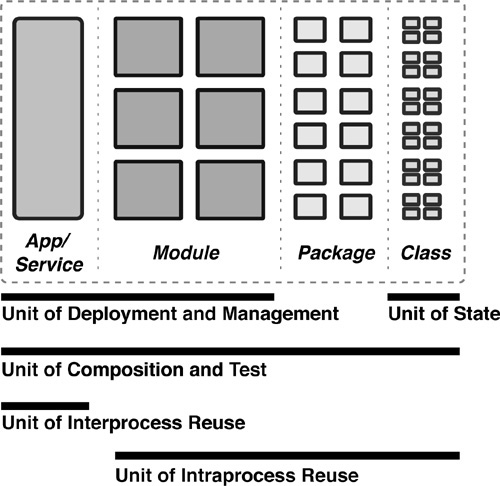
\includegraphics[width=0.8\textwidth]{module.jpeg}
\caption{Module definition diagram}
\label{fig:module}
\end{figure}

Figure \ref{fig:module} illustrates this defnition and all the individual aspects of a module \cite{Knoernschild:2012}:

\subsection{OSGi}
\gls{OSGi} is the most widely used and highly developed module system and service platform for the Java environment. This chapter aims to show why \gls{OSGi} is the best choice for building highly modular Java-based software systems as it supports all requirements of modularity defined by \citeauthor{Knoernschild:2012}\cite{Knoernschild:2012}.

The \gls{OSGi} technology is a set of specifications that define a dynamic component system for Java. These specifications enable a development model where applications are dynamically composed of many different reusable components. The \gls{OSGi} specifications enable modules to hide their implementations from other modules while communicating through services, which are objects that are specifically shared between modules. This surprisingly simple model has far reaching effects for almost any aspect of the software development process \cite{OSGi}. In \gls{OSGi} parlance, a module is known as a bundle. \gls{OSGi} provides a framework for managing bundles that are packaged as regular Java JAR files with an accompanying manifest. The manifest contains important metadata that describes the bundles and its dependencies to the \gls{OSGi} framework \cite{Knoernschild:2012}. Figure \ref{fig:layering-osgi} shows the layered model architecture of the \gls{OSGi} service platform.

\begin{figure}[H]
\centering
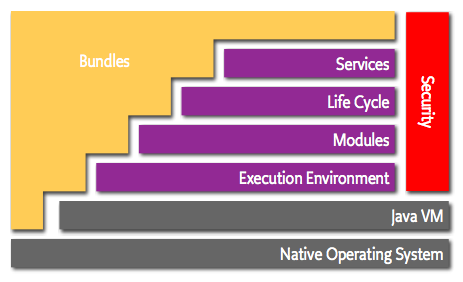
\includegraphics[width=0.73\textwidth]{layering-osgi.png}
\caption{\gls{OSGi} layered model \cite{OSGi}}
\label{fig:layering-osgi}
\end{figure}

\subsubsection{Implementations}
\gls{OSGi} is the foundation for many different Application Servers and IDEs. Some of the most widely used open source implementations of the \gls{OSGi} specification are listed here: 

\begin{itemize}
	\item \textbf{Eclipse Equinox} \\
		\url{http://eclipse.org/equinox/} \\
		Equinox is the core of the plug-in runtime for the Eclipse IDE.
	\item \textbf{Apache Felix} \\
		\url{http://felix.apache.org/} \\
		Apache Felix is the open source \gls{OSGi} implementation powered by the \gls{ASF} and is the basis of several other Apache projects like Apache Aries and Apache Karaf.
	\item \textbf{Knopflerfish} \\
		\url{http://www.knopflerfish.org/} \\
		Knopflerfish is the spin-off from one of the \gls{OSGi} alliance founding members and was open-sourced in 2003.
\end{itemize}

The developed framework uses Apache Felix for bundle testing purposes but aims to be \gls{OSGi} compliant and implementation independence. Apache Felix was chosen for its easy configuration and small memory footprint.

\subsection{Relevant patterns}
\subsubsection{Dependency Injection}
\gls{DI} is an expression introduced by Martin Fowler in its article \textit{Inversion of Control Containers and the Dependency Injection Pattern} \cite{Fowler:2004}. Dependency Injection specifies the means for obtaining objects in such a way as to maximize reusability, testability and maintainability compared to traditional approaches such as constructors, factories, and service locators \cite{JSR330}. \gls{DI} does this by allowing a class to specify its dependencies and rely on their provision at runtime rather than retrieving them explicitly. This leaves the programmer's code clean, flexible, and relatively free of dependency-related infrastructure \cite{JSR330}.

\fxfatal{Put into context with modularity}
% Modularity is very concerned with dependency management, DI is a good way to embrace it

\subsubsection{Single Responsibility Principle}
\fxfatal{Content and context}

\subsubsection{Dependency Inversion Principle}
\fxfatal{Content and context}

\subsection{Supporting libraries and tools}
\fxfatal{Introduction}
% Relation to modularity and my work!

\subsubsection{Guice}
Guice is a lightweight dependency injection framework for Java \cite{Guice}. It's Open Source and available on \url{https://code.google.com/p/google-guice/}.

The typical code to implement Guice is shown in the following two listings. The first shows a simple \textit{Module}. Modules in Guice are usually used to bind interfaces to concrete classes.

\begin{listing}[H]
\begin{minted}{java}
public final class ProcessModule extends AbstractModule {

    @Override 
    protected void configure() {
        bind(ProcessService.class).to(DefaultProcessService.class);
    }

}
\end{minted}
\caption{Guice module}
\end{listing}

In your classes you usually define a single constructor, annotated with \texttt{@Inject}, and all required dependencies as parameters. The construction of instances and the dependency resolution is done by Guice, no additional boilerplate code is necessary.

\begin{listing}[H]
\begin{minted}{java}
final class DefaultEngine implements Engine {

    private final ProcessService service;

    @Inject
    DefaultEngine(ProcessService service) {
        this.service = service;
    }

}
\end{minted}
\caption{Constructor injection}
\end{listing}

\subsubsection{Guice Extensions}
Guice has an extensible plug-in mechanism which allows third parties to provide additional functionality. Banshie uses two official Guice extension extensively: Assisted Inject\footnote{\url{https://code.google.com/p/google-guice/wiki/AssistedInject}} and Multibindings\footnote{\url{https://code.google.com/p/google-guice/wiki/Multibinding}}. Assisted Inject allows the combination of Guice-provided dependencies and user-provided parameters on a single injection point. Multibindings supports the binding and injection of Sets and Maps.

\paragraph{Peaberry}
Guice has no native OSGi support, apart from maybe the OSGi-compatible bundle manifest. To overcome this shortcoming, Peaberry\footnote{\url{https://code.google.com/p/peaberry/}}, a third-party open-source Guice extension, offers OSGi-Guice bridge capabilities. It offers \gls{DI} of OSGi dynamic services via Guice's common injection mechanisms and provides a rich and typesafe API to deal with the OSGi service registry and lifecycle events. Listing \ref{lst:peaberry-lifecycle} shows the usage of Peaberry's lifecycle annotations.

\begin{listing}[H]
\begin{minted}{java}
import org.ops4j.peaberry.activation.Start;

public class DefaultCorpusRepository implements CorpusRepository {

    private File basePath = new File("corpora");

    @Start
    public void onStart() {
        basePath.mkdirs();
    }

}
\end{minted}
\caption{Peaberry lifecycle annotation}
\label{lst:peaberry-lifecycle}
\end{listing}

Peaberry even supports the automatic \gls{DI} context creation upon bundle start by using an OSGi extender bundle. Bundles just need to provide the following bundle header to trigger an execution:

\begin{listing}[H]
\texttt{Bundle-Module: org.whiskeysierra.banshie.execution.ExecutionModule}
\caption{Peaberry bundle header}
\end{listing}

Peaberry creates one \texttt{Injector} per bundle, any interaction between bundles is based on standard OSGi services, which allows to combine Peaberry-aware bundles and normal ones.

\subsubsection{BND Tool and the Maven Bundle Plugin}
With \gls{OSGi} you are forced to provide additional metadata in the JAR's manifest to verify the consistency of your classpath. This metadata must be closely aligned with the class files in the bundle. Maintaining this metdata is an error prone chore because many aspects are redundant. The core task of the BND Tool is to analyze the class files and find every dependency. These dependencies are then merged with instructions supplied by the user \cite{BND}. Since Banshie uses Apache Maven for building its independent modules, the natural choice was to use a Maven Plugin for this, which is provided by the Apache Felix Maven Bundle Plugin \footnote{\url{http://felix.apache.org/site/apache-felix-maven-bundle-plugin-bnd.html}}. The following listing shows the bare minimum of configuration code to use the Maven Bundle Plugin in a POM file.

\begin{listing}[H]
\begin{minted}{xml}
<packaging>bundle</packaging>
...
<build>
    <plugins>
        <plugin>
            <groupId>org.apache.felix</groupId>
            <artifactId>maven-bundle-plugin</artifactId>
        </plugin>
    </plugins>
</build>
\end{minted}
\caption{Maven Bundle Plugin usage}
\end{listing}


\subsection{Summary}
\gls{OSGi} is considered to be the most advanced module system for the Java platform. It supports all aspects of modularity, such as deployability, manageability, reusability and composability. Since modularity and its benefits and advantages, such as maintainability, is one of the main requirement of this work, \gls{OSGi} is the best choice as a foundation for the framework.

\fxfatal{Relates to my work how?}
\section{Related Work}
\label{sec:related-work}
This chapter aims to provide a quick overview of some of the better known frameworks for evaluating information extraction systems.

\fxfatal{Discuss each system individually in the context of this thesis}

\subsection{Evaliex}
\textit{Evaliex} is an \gls{IE} evaluation tool which integrates measurement concepts, like state-of-the-art scoring metrics, measuring string and semantic similarities and by parameterization of metric scoring, and provides an efficient user interface that supports evaluation control and the visualization of \gls{IE} results.

To guarantee domain independence, the tool additionally provides a Generic Mapper for XML Instances (GeMap) that maps domain-dependent XML files containing \gls{IE} results to generic ones. Compared to other tools, it provides more flexible testing and better visualization of extraction results for the comparison of different (versions of) information extraction systems \cite{Feilmayr:2012}.

\textit{Evaliex}  was part of a master thesis by \citeauthor{Linsmayr:2010} in 2010: \citetitle{Linsmayr:2010} \cite{Linsmayr:2010}. A corresponding paper was published by \citeauthor{Feilmayr:2012} later in 2012: \citetitle{Feilmayr:2012} \cite{Feilmayr:2012}.

Although Evaliex is a promising tool with a rich feature set; it's not available for other parties, as neither the tool itself nor the source code has yet been published. Evaliex also lacks a proper \gls{API} as it is purely designed to be a standalone desktop application providing a Java-based user interface.

\subsection{GATE}
The \gls{GATE}\footnote{\url{http://gate.ac.uk/}} is a Free \& Open-Source infrastructure for developing and deploying software components that processes human language. It is more than 15 years old and in active use for all types of computational tasks involving language. GATE excels at text analysis of all shapes and sizes. \cite{Cunningham:2011}.

The evaluation in GATE is provided by a component called the \textit{AnnotationDiff Tool} which compares the individual annotations of a hypothesis with a reference. The differences are listed and visualized in color. GATE calculates the metrics recall, precision and F-measure \cite{Linsmayr:2010}.

Similar to Evaliex the GATE Annotation Diff Tool only supports a graphical user interface and is not designed to be embedded in or used by other systems. The tool also lacks error measures, by name error measure, error per response fill and slot error rate.

\subsection{Ellogon}
Ellogon\footnote{\url{http://www.ellogon.org/}} is a multi-lingual, cross-platform, general-purpose language engineering environment, developed in order to aid both researchers who are doing research in computational linguistics, as well as companies who produce and deliver language engineering systems. Ellogon as a language engineering platform offers an extensive set of facilities, including tools for processing and visualising textual/HTML/XML data and associated linguistic information, support for lexical resources (like creating and embedding lexicons), tools for creating annotated corpora, accessing databases, comparing annotated data, or transforming linguistic information into vectors for use with various machine learning algorithms \cite{Ellogon}.

The deviation calculation of two collections of documents is provided by the \textit{Collection Comparison tool}. It compares the annotations and attributes. After association it calculates precision, recall and F-measure \cite{Linsmayr:2010}.

The Ellogon Collection Comparison tool ships, very much like the Gate Annotation Diff Tool, only with a graphical user interface and lacks an API and the possibility to be embedded in other tools as a library. Ellogon also only supports the performance figures precision, recall and F-measure.

\subsection{ANNALIST}
\gls{ANNALIST}\footnote{\url{http://annalist.sourceforge.net/}} is a scoring system for the evaluation of the output of semantic annotation systems. ANNALIST has been designed as a system that is easily extensible and configurable for different domains, data formats, and evaluation tasks. The system architecture enables data input via the use of plugins and the users can access the system’s internal alignment and scoring mechanisms without the need to convert their data to a specified format. Although developed for evaluation tasks that involve the scoring of entity mentions and relations primarily, ANNALIST's generic object representation and the availability of a range of criteria for the comparison of annotations enable the system to be tailored to a variety of scoring jobs \cite{Demetriou:2008}.

ANNALIST is, in contrast to the previously described systems, a pure evaluation tool. The data can be imported via special plug-ins and is processed by individual modules. The \textit{Alignment Tool} associates hypotheses and references for each annotation type. The subsequent metric calculation is performed by the scoring module which determines precision, recall and the F-measure. The output module visualizes the results in a table \cite{Linsmayr:2010}.

\fxfatal{Shortcomings?}

\subsection{Summary}
\fxfatal{Shortcomings of these systems? What does Banshie try to improve?}
% all tools are just evaluating results, they don't handle execution and can't evaluate runtime performance

\section{Design}
\label{sec:design}

This chapter presents the implemented framework \textit{Banshie} (Benchmark Framework for Information Extraction). The requirements, architecture, design and concrete implementation details are explained and discussed on the following pages.

\subsection{Analysis and requirements}
The main goal was to provide a platform to benchmark domain-specific information extraction modules. The framework had to be designed for extension and modularity. It should be based on the OSGi infrastructure and build with state-of-the-art patterns, like \gls{DI}, \gls{IoC} and Composition over Inheritence in mind.

Since Banshie had to be developed in an Open Source fashion, its whole code base as well as the  documentation is available via

\url{https://github.com/whiskeysierra/banshie}

\fxfatal{Integration into bigger platform, future development by other researchers/programmers, ...}

\subsection{Architecture}
Banshie is completely written in Java and distributed as OSGi bundles. The architecture of the framework was not the result of a \gls{BDUF} but is rather based on a very rough design idea which allows to incrementally build in the design details as the project progresses. \citeauthor{Knoernschild:2012} provides a catalog of architectural patterns for building highly modular systems in his book: \citetitle{Knoernschild:2012} \cite{Knoernschild:2012}

Almost all Banshie's modules are the result of applying these patterns during the development. The following figure shows all relevant modules as well as their dependencies.

\newpage
\begin{figure}[H]
\centering
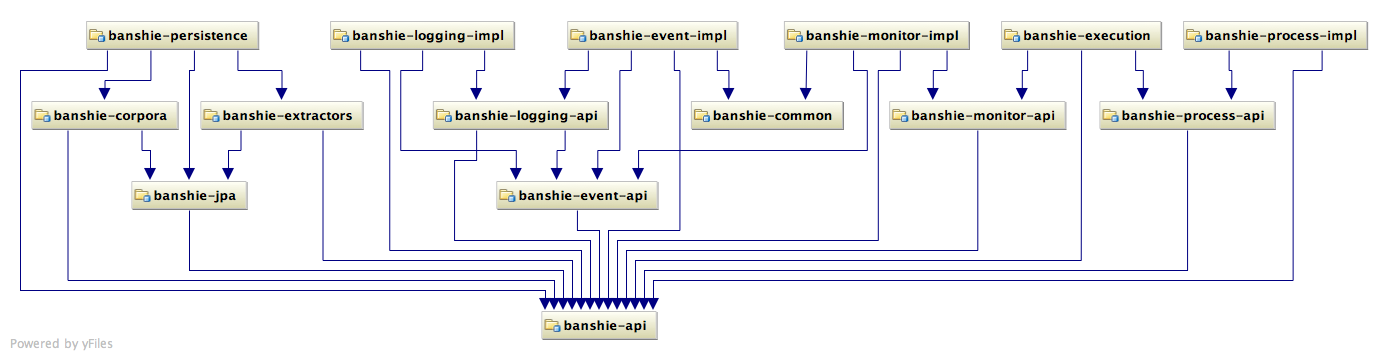
\includegraphics[angle=90, width=0.38\textwidth]{module-dependencies.png}
\caption{Module dependencies}
\label{fig:module-dependencies}
\end{figure}

\newpage
\subsection{Technologies and patterns}

\subsubsection{Dependency Injection}
\gls{DI} is an expression introduced by Martin Fowler in its article \textit{Inversion of Control Containers and the Dependency Injection Pattern} \cite{Fowler:2004}. Dependency Injection specifies the means for obtaining objects in such a way as to maximize reusability, testability and maintainability compared to traditional approaches such as constructors, factories, and service locators \cite{JSR330}. \gls{DI} does this by allowing a class to specify its dependencies and rely on their provision at runtime rather than retrieving them explicitly. This leaves the programmer's code clean, flexible, and relatively free of dependency-related infrastructure \cite{JSR330}.

\paragraph{Guice}
Guice is a lightweight dependency injection framework for Java \cite{Guice}. It's Open Source and available on \url{https://code.google.com/p/google-guice/}.

The typical code to implement is shown in the following two listings. The first shows a simple \textit{Module}. Modules in Guice are usually used to bind interfaces to concrete classes.

\begin{listing}[H]
\begin{minted}{java}
public final class ProcessModule extends AbstractModule {

    @Override 
    protected void configure() {
        bind(ProcessService.class).to(DefaultProcessService.class);
    }

}
\end{minted}
\caption{Guice module}
\end{listing}

In your classes you usually define a single constructor, annotated with \texttt{@Inject}, and all required dependencies as parameters. The construction of instances and the dependency resolution is done by Guice, no additional boilerplate code is necessary.

\begin{listing}[H]
\begin{minted}{java}
final class DefaultEngine implements Engine {

    private final ProcessService service;

    @Inject
    DefaultEngine(ProcessService service) {
        this.service = service;
    }

}
\end{minted}
\caption{Constructor injection}
\end{listing}

\paragraph{Guice Extensions}
Guice has an extensible plug-in mechanism which allows third parties to provide additional functionality. Banshie uses two official Guice extension extensively: Assisted Inject\footnote{\url{https://code.google.com/p/google-guice/wiki/AssistedInject}} and Multibindings\footnote{\url{https://code.google.com/p/google-guice/wiki/Multibinding}}. Assisted Inject allows the combination of Guice-provided dependencies and user-provided parameters on a single injection point. Multibindings supports the binding and injection of Sets and Maps.

\paragraph{Peaberry}
Guice has no native OSGi support, apart from maybe the OSGi-compatible bundle manifest. To overcome this shortcoming, Peaberry\footnote{\url{https://code.google.com/p/peaberry/}}, a third-party open-source Guice extension offers OSGi-Guice bridge capabilities. It offers \gls{DI} of OSGi dynamic services via Guice's common injection mechanisms and provides a rich and typesafe API to deal with the OSGi service registry and lifecycle events. Listing \ref{lst:peaberry-lifecycle} shows the usage of Peaberry's lifecycle annotations.

\begin{listing}[H]
\begin{minted}{java}
import org.ops4j.peaberry.activation.Start;

public class DefaultCorpusRepository implements CorpusRepository {

    private File basePath = new File("corpora");

    @Start
    public void onStart() {
        basePath.mkdirs();
    }

}
\end{minted}
\caption{Peaberry lifecycle annotation}
\label{lst:peaberry-lifecycle}
\end{listing}

Peaberry even supports the automatic \gls{DI} context creation upon bundle start by using an OSGi extender bundle. Bundles just need to provide the following bundle header to trigger an execution:

\begin{listing}[H]
\texttt{Bundle-Module: org.whiskeysierra.banshie.execution.ExecutionModule}
\caption{Peaberry bundle header}
\end{listing}

Peaberry creates one \texttt{Injector} per bundle, any interaction between bundles is based on standard OSGi services, which allows to combine Peaberry-aware bundles and normal ones.

\subsubsection{Persistence}
Banshie's persistence layer is based on the \gls{JPA} 2.0 Standard. \gls{JPA} allows to build modules without hardcoding for a specific persistence provider or database vendor. Thus allowing to swap implementations later in the development lifecycle without the need to rewrite large portions of the code base. Banshie uses Apache OpenJPA as a \gls{JPA} provider and Apache Derby as the underlying database. Derby is a \gls{RDBMS} written in Java and is distributable as a single Jar file and can be embedded in other applications rather easily.

Using \gls{JPA} in an \gls{OSGi} environment is not a straight forward task. \gls{OSGi} requires bundles to run in different and independent class loaders, while \gls{JPA} heavily relies on classpath scanning and reflection. Both techniques don't work quite well together. Because \gls{JPA}-based persistence is a common requirement, the \citetitle{OSGI:Enterprise} addressed this issue and specifies a standard way to define \textit{Persistence} and \textit{Client bundles} \cite{OSGI:Enterprise}. A persistence bundle is a bundle with the following bundle header:

\begin{listing}[H]
\texttt{Meta-Persistence: META-INF/persistence.xml}
\caption{Persistence bundle header}
\end{listing}

A client bundle is just a bundle that makes use of the \texttt{EntityManagerFactory} provided by the corresponding persistence unit. Most \gls{OSGi} containers delegate this part of the \gls{OSGi} specification to third-party libraries and bundles. Apache Aries aims to provide portable implementations in form of standard \gls{OSGi} bundles for those parts of the \gls{OSGi} specification. Banshie uses the JPA module of Apache Aries consisting of \textit{Aries JPA API bundle} and the \textit{Aries JPA container bundle}. To minimize common boilerplate code and manual transaction handling, all \gls{JPA} client bundles use the Guice extension \textit{Guice Persist}. Guice Persist offers AOP-interception for annotated methods as shown in the following listing:

\begin{listing}[H]
\begin{minted}{java}
class DefaultCorpusRepository implements CorpusRepository {

    private EntityManager manager() {
        return provider.get();
    }

    @Transactional
    @Override
    public Corpus get(UUID uuid) {
        return manager().find(CorpusEntity.class, uuid);
    }

}
\end{minted}
\caption{Guice Persist annotation}
\end{listing}

\subsubsection{Build tools}
\paragraph{BND Tool and the Maven Bundle Plugin}
With \gls{OSGi} you are forced to provide additional metadata in the JAR's manifest to verify the consistency of your classpath. This metadata must be closely aligned with the class files in the bundle. Maintaining this metdata is an error prone chore because many aspects are redundant. The core task of the BND Tool is to analyze the class files and find any dependencies. These dependencies are then merged with instructions supplied by the user \cite{BND}. Since Banshie uses Apache Maven for building its independent modules, the natural choice was to use a Maven Plugin for this, which is provided by the Apache Felix Maven Bundle Plugin \footnote{\url{http://felix.apache.org/site/apache-felix-maven-bundle-plugin-bnd.html}}. The following listing shows the bare minimum of configuration code to use the Maven Bundle Plugin in a POM file.

\begin{listing}[H]
\begin{minted}{xml}
<packaging>bundle</packaging>
...
<build>
    <plugins>
        <plugin>
            <groupId>org.apache.felix</groupId>
            <artifactId>maven-bundle-plugin</artifactId>
        </plugin>
    </plugins>
</build>
\end{minted}
\caption{Maven Bundle Plugin usage}
\end{listing}

\newpage
\subsection{API}
The framework's \gls{API} can be divided into three main components which are described in detail on the following pages.

\paragraph{Domain model and persistence}
Banshie's domain model has been designed with simplicity and extensibility in mind. The two only entity classes, \texttt{Corpus} and \texttt{Extractor}, are merely containers for file locations and very little meta data, but since the persistence layer is based on \gls{JPA}, which is based on \textit{Plain Old Java Objects}, adding properties is a rather easy task.

An extractor holds the name, version and the path to the executable jar file while a corpus identifies the reference output as well as a related input document.

For each of the model classes a persistence service interface is provided. Since the framework in it current stage does not require very sophisticated features, the interface of these services is kept to a minimum intentionally.

\begin{figure}[H]
\centering
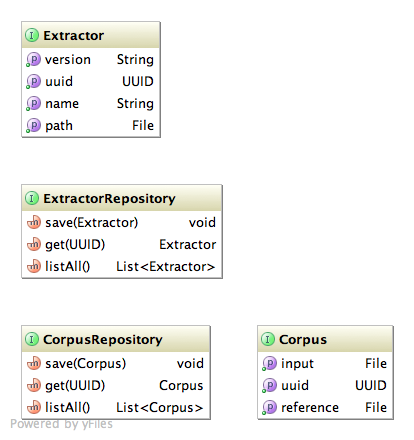
\includegraphics[width=0.8\textwidth, trim=20px 20px 0 0, clip=true]{api-model.png}
\caption{Banshie model and persistence API}
\end{figure}

\newpage
\paragraph{Execution}
Apart from the domain model and persistence layer, the framework offers two significant features to its clients: execution and evaluation. The execution package contains one major interface for executing extractors: the \texttt{Engine}. The Engine provides a single methods which takes an Extractor-Corpus-pair and performs an execution. The result of the extractor run is than passed back to the caller in form of a \texttt{ExtractorResult} containing references to the extractor's xml output file and the event log file. For more details about the structure of the event log file please consult chapter \ref{sec:implementation}.

\begin{figure}[H]
\centering
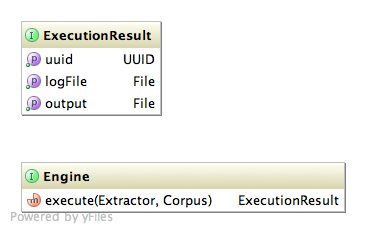
\includegraphics[width=0.7\textwidth, trim=20px 20px 0 0, clip=true]{api-execution.png}
\caption{Banshie Execution API}
\end{figure}

\newpage
\paragraph{Evaluation}
Evaluation is, next to execution, the other main feature of the framework.

\fxfatal{Reasons to do execution and evaluation in two different steps!}
% memory efficiency, later re-evaluation using different evaluators/configurations

The evaluation packages contains several type definitions as shown in figure \ref{fig:evaluation-api}:

\begin{figure}[H]
\centering
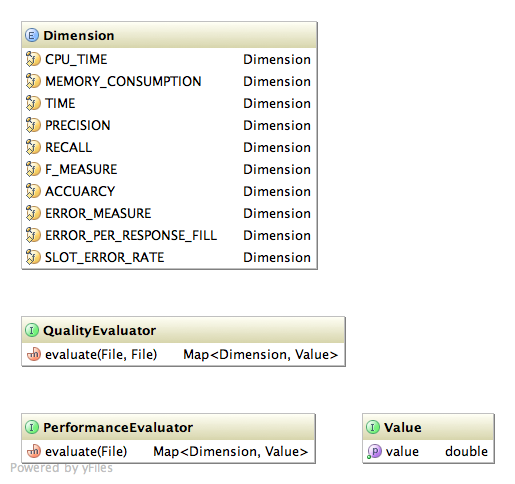
\includegraphics[width=0.8\textwidth, trim=20px 19px 0 0, clip=true]{api-evaluation.png}
\caption{Banshie Evaluation API}
\label{fig:evaluation-api}
\end{figure}

The two main service types are \texttt{QualityEvaluator} and \texttt{PerformanceEvaluator}. Both have a very similar interface, since they provide a single method to evaluate the execution result. The QualityEvaluator compares the Corpus' reference and the Extractor's hypothesis and calculates quality performance measures like Precision, Recall and F-Measure. The PerformanceEvaluator on the other hand focuses on calculating runtime performance measure, like CPU time, memory consumption and execution time by processing the event log file.

\newpage
\paragraph{API Usage}
Listing \ref{lst:usage} shows the simple basic steps required to perform a single extractor execution and evaluation.

\begin{listing}[H]
\begin{minted}{java}
// via dependency injection or direct instantiation
final ExtractorRepository extractors = ...;
final CorpusRepository corpora = ...;
final Engine engine = ...;
final PerformanceEvaluator performance = ...;
final QualityEvaluator quality = ...;

final Extractor extractor = extractors.get(extractorId);
final Corpus corpus = corpora.get(corpusId);

final ExecutionResult result = engine.execute(extractor, corpus);
final Map<Dimension, Value> p = 
    performance.evaluate(result.getLogFile());
final Map<Dimension, Value> q = 
    quality.evaluate(corpus.getReference(), result.getOutput());

// handle evaluation results
...
\end{minted}
\caption{Banshie API usage}
\label{lst:usage}
\end{listing}

\subsection{Extractor interface specification}
Since Banshie aims to evaluate the extraction quality as well as the runtime performance of information extraction systems it sets some special requirements for extractors.

Any extractor evaluated by the framework is required to by written in Java and compiled for Java 1.6 or higher as a single executable Jar file. Being packaged as a single file requires the extractor to bundle every external dependency into a single archive. Embedding third-party java libraries can be accomplished by utilizing the \textit{JarJar}\footnote{\url{https://code.google.com/p/jarjar/}} tool. External files like models and training data can packaged as standard classpath resources.

For a Jar file to be executable it has to have a manifest file, i.e. META-INF/MANIFEST.MF), and a manifest header as shown in the following listing:

\begin{listing}[H]
\texttt{Main-Class: org.whiskeysierra.banshie.example.opennlp.Main}
\caption{Extractor manifest header}
\end{listing}

The extractor can than be started using the following command: \\ \texttt{java -jar extractor.jar}

Since an extractor under evaluation has a single input, the test document, and a single output, the annotated hypothesis, the natural choice was to utilize standard streams, standard input (\textit{stdin}) and and standard output (\textit{stdout}) respectively. The test document is passed to the extractor as plain text in UTF-8 encoding. Whether the extractor streams the document or reads it into memory as a whole is up the extractor. The output format is \gls{XML} as defined by the schema shown in listing \ref{lst:xml-schema}.

\fxfatal{Does only support single document extraction!}

\begin{listing}[H]
\inputminted{xml}{../../../../../banshie-api/src/main/resources/schema.xsd}
\caption{Banshie XML Schema}
\label{lst:xml-schema}
\end{listing}

As shown in listing \ref{lst:xml-example}, the defined output format is a very simple XML document containing the original document and all found entities annotated with the corresponding type as a simple XML element tag.

\begin{listing}[H]
\inputminted{xml}{../../../../../banshie-api/src/main/resources/example.xml}
\caption{Banshie XML Example}
\label{lst:xml-example}
\end{listing}

The span element has three attributes: \texttt{type}, \texttt{start} and \texttt{end}. Type is one of \texttt{person}, \texttt{organization}, \texttt{date} or \texttt{location}, based on the ENAMEX tags developed for the Message Understanding Conference \cite{Grishman:1996}.

The attribtues \texttt{start} and \texttt{end} define the UTF-8 character offset of the span in the original document to support character based association of spans in the reference and the predication.

\subsection{Reference-hypothesis association}
\label{sec:association}
Evaliex \cite{Linsmayr:2010} uses an extended version of the \enquote{General Greedy Mapping Algorithm} as proposed by \citeauthor{Douthat:1998} in 1998 \cite{Douthat:1998}. It's based on finding matching pairs of spans in the reference and the predication based on string or word similarity algorithms like Levenshtein-distance or the Jaccard-coeffecient. But since Banshie, in its current version, focuses solely on Named Entity Recognition, a simpler algorithm to associate reference and hypothesis has been used. Spans are matched based on character offsets calculated from the original document. This way an extractor is required to find exact or partial matches of spans defined in the reference to score in the evaluation metrics.
\fxfatal{Don't start with Evaliex}

\subsection{Implementation}
\label{sec:implementation}

\subsubsection{Engine}
The \textit{Engine} interface offers a single facade to executing an \texttt{Extractor} against a supplied \texttt{Corpus}. It's the Engine's responibility to provide an independent and isolated execution environment for extractors, to manage process creation and lifecycle and to collect and persist runtime events.

After an initial design draft, it was clear, that the Engine implementation will be too big for a single module. So the engine implementation was split up into multiple smaller, more maintainable modules using the module development patterns defined by \citeauthor{Knoernschild:2012}\cite{Knoernschild:2012} and discussed in chapter \ref{sec:modularity}. The engine's submodules are described in the following chapters.

\begin{figure}[H]
\centering
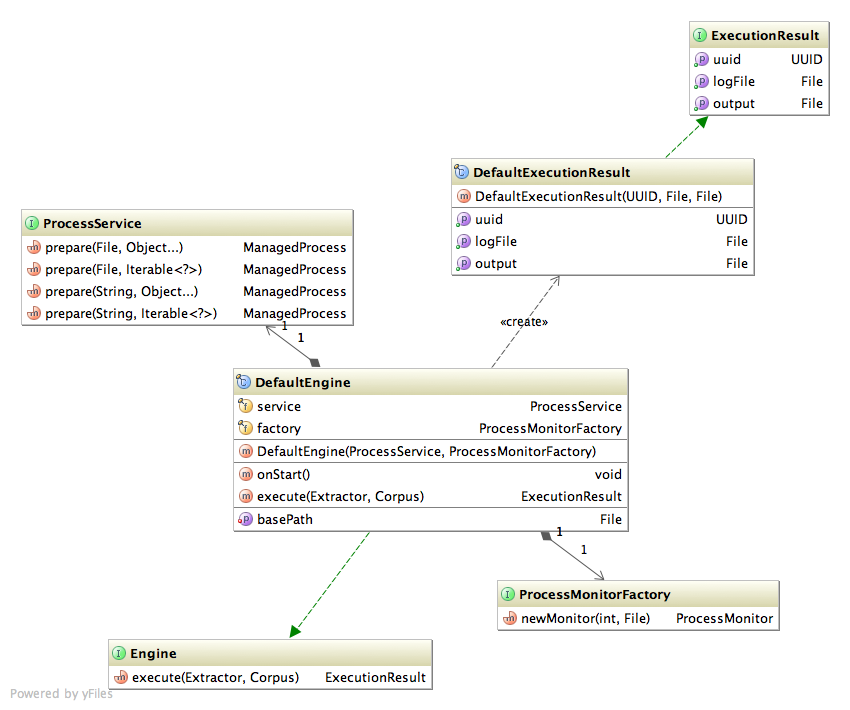
\includegraphics[width=\textwidth, trim=20px 20px 0 0, clip=true]{execution.png}
\caption{Engine implementation}
\end{figure}

\newpage
\paragraph{Process management}
The Java Process API is part of the Java Runtime Environment since version 1.0 but it has several  pitfalls and unfortunately there are a lot of common traps \cite{Cartmell:2009}. \fxfatal{Examples?} There even has been filed a \gls{JEP} to improve the API for controlling and managing operating system processes. \cite{JEP:102}.

Since executing an extractor in an isolated, independent execution environment is a crucial part of the Engine's task the framework required a cleaner, more fail-safe API for process creation and lifecycle management that integrates nicely with the rest of the framework and it's main general purpose library, i.e. Guava. Listing \ref{lst:process} demonstrates the minimal steps to use the  framework's Process API while figure \ref{fig:process} shows the relevant parts of it.

\begin{listing}[H]
\begin{minted}{java}
final ManagedProcess managed = service.prepare("java", "-version");
final RunningProcess process = managed.call();

// write to process.getOutput() or
// read from process.getInput()

process.await();
// or process.cancel()
\end{minted}
\caption{ProcessService API example usage}
\label{lst:process}
\end{listing}

\begin{figure}[H]
\centering
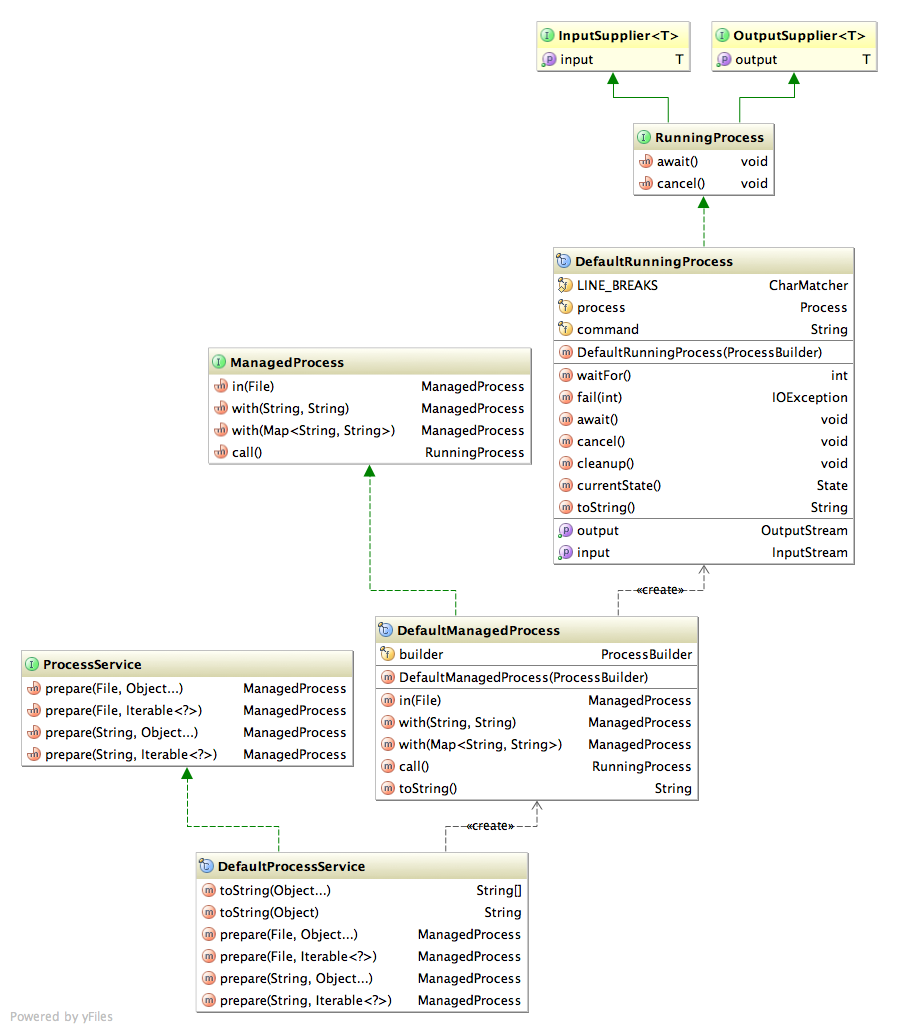
\includegraphics[width=\textwidth, trim=20px 20px 0 0, clip=true]{process.png}
\caption{ProcessService implementation}
\label{fig:process}
\end{figure}

\newpage
\paragraph{Process monitoring}
After an extractor has been started in its own environment using the ProcessService API, the operating system process needs to be monitored to ensure correct execution and to collect events, like current CPU time and memory consumption, in a periodical way, e.g. every x milliseconds.

\begin{figure}[H]
\centering
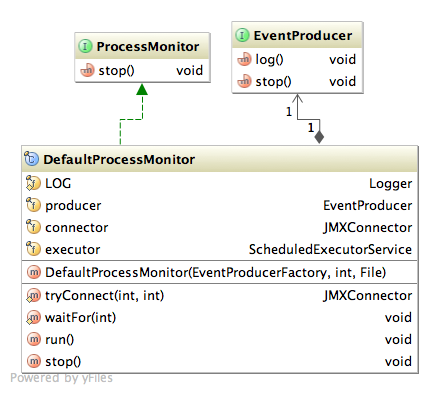
\includegraphics[width=0.8\textwidth, trim=20px 20px 0 0, clip=true]{monitor.png}
\caption{ProcessMonitor implementation}
\end{figure}

The repeated polling is realized with the JDK's built-in \\ \texttt{ScheduledExecutorService}\footnote{\url{http://docs.oracle.com/javase/6/docs/api/java/util/concurrent/ScheduledExecutorService.html}} which schedules a special \texttt{Runnable} to run in a scheduled fashion, like shown in listing \ref{lst:scheduling}

\fxfatal{Mention the possible impact of JMX/Polling auf die Messergebnisse: context switches}
\fxfatal{Possible solution: multiple runs and calculate the average}

\begin{listing}[H]
\begin{minted}{java}
executor.scheduleAtFixedRate(runnable, 0L, 1L, TimeUnit.SECONDS);
\end{minted}
\caption{Scheduling in java}
\label{lst:scheduling}
\end{listing}

\newpage
Collecting events on a separate process can be realized by using \gls{JMX}, which allows managing and monitoring java applications through a well specified and extensible interface. To allow a \gls{JMX} connection, a java process needs to be started with a special set of command line parameters as shown in listing \ref{lst:process-configuring}.

\begin{listing}[H]
\begin{minted}{java}
final ManagedProcess managed = service.prepare(
    "java",
    "-Dcom.sun.management.jmxremote",
    "-Dcom.sun.management.jmxremote.port=" + port,
    "-Dcom.sun.management.jmxremote.authenticate=false",
    "-Dcom.sun.management.jmxremote.ssl=false",
    "-jar", extractor.getPath()
);
\end{minted}
\caption{Configuring process to use JMX}
\label{lst:process-configuring}
\end{listing}

\fxfatal{Mention that this is the reason why Banshie is limited to JVM-based extractors at the moment.}

After the process has been started, a \gls{JMX} connection can be established with the following steps:

\begin{listing}[H]
\begin{minted}{java}
final String url = "service:jmx:rmi:///jndi/rmi://localhost:" + 
    port + "/jmxrmi";
final JMXServiceURL serviceUrl = new JMXServiceURL(url);
final JMXConnector connector = 
    JMXConnectorFactory.connect(serviceUrl, null);
\end{minted}
\caption{JMX connection}
\label{lst:jmx}
\end{listing}

The default implementation of the \texttt{ProcessMonitor} interface delegates the work of creating events to another service, the \texttt{EventProducer}, by passing on the \texttt{JMXConnector}.

\newpage
\paragraph{Event production}
\begin{figure}[H]
\centering
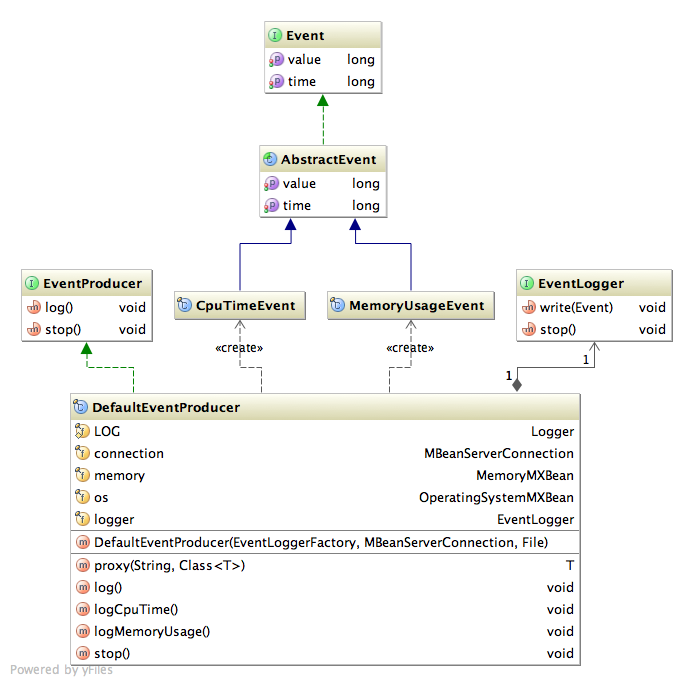
\includegraphics[width=\textwidth, trim=20px 20px 0 0, clip=true]{event.png}
\caption{EventProducer implementation}
\end{figure}

It's the \texttt{EventProducer}'s responsibility to retrieve runtime performance figures by calling the corresponding \gls{JMX} endpoints, to create and populate the suitable \texttt{Event} instances. The producer creates \gls{JMX} proxies for \texttt{MemoryMXBean}\footnote{\url{http://docs.oracle.com/javase/6/docs/api/java/lang/management/MemoryMXBean.html}} and \texttt{OperatingSystemMXBean}\footnote{\url{http://docs.oracle.com/javase/6/docs/jre/api/management/extension/com/sun/management/OperatingSystemMXBean.html}}, creates \texttt{CpuTimeEvent}s and \texttt{MemoryUsageEvent}s and delegates their persistence to the \texttt{EventLogger} service.

\paragraph{Event persistence}
Once events have been created, they need to be persisted on the file system to allow processing them later on during evaluation. Event persistence in Banshie is provided by the default \texttt{EventLogger} implementation, which creates a single text-oriented log file. \texttt{Event}s are serialized using \gls{JSON} mapping capabilities of the Jackson\footnote{\url{http://jackson.codehaus.org/}} library. The resulting event log file contains one \gls{JSON} entity per line.

\fxfatal{Why not JPA? Advantages of JSON? Versioning!}

\begin{figure}[H]
\centering
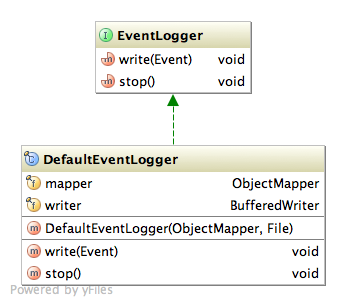
\includegraphics[width=0.65\textwidth, trim=20px 19px 0 0, clip=true]{logging.png}
\caption{EventLogger implementation}
\end{figure}

\begin{listing}[H]
\begin{minted}{javascript}
{"type":"cpu","time":1362134570374,"value":440000000}
{"type":"memory","time":1362134570376,"value":12817008}
{"type":"cpu","time":1362134571374,"value":440000000}
{"type":"memory","time":1362134571375,"value":12818096}
{"type":"cpu","time":1362134572378,"value":440000000}
{"type":"memory","time":1362134572393,"value":12822128}
\end{minted}
\caption{Example event log file excerpt}
\label{lst:event-log}
\end{listing}

\newpage
\subsubsection{Quality evaluation}
The default \texttt{QualityEvaluator} implementation has serveral tasks. It needs to map the prediction to the reference, count true positives, false positives, false negatives, run configured scoring metrics and collect their results.

\begin{figure}[H]
\centering
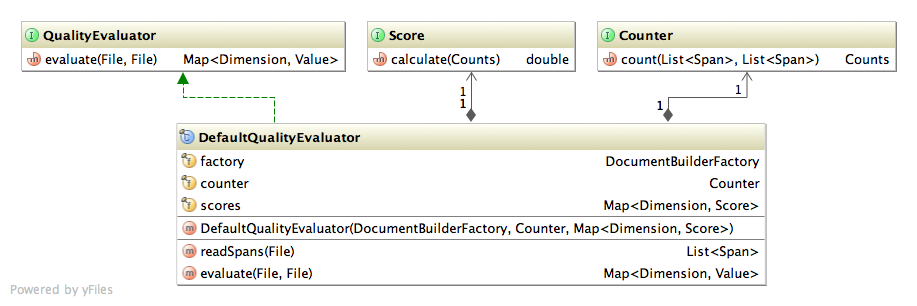
\includegraphics[width=\textwidth, trim=20px 20px 0 0, clip=true]{quality-evaluation.png}
\caption{QualityEvaluator implementation}
\end{figure}

The reference-hypothesis association is provided by the \texttt{Counter} class, as shown in figure \ref{fig:counter}. For details about the reference-hypothesis association algorithm used, please consult chapter \ref{sec:association}.

\begin{figure}[H]
\centering
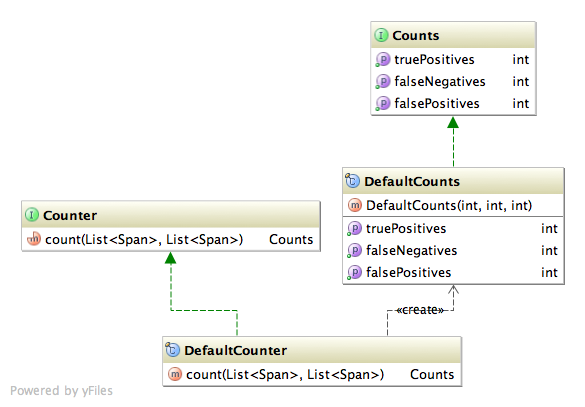
\includegraphics[width=0.8\textwidth, trim=20px 20px 0 0, clip=true]{counter.png}
\caption{Counter implementation}
\label{fig:counter}
\end{figure}

The scoring metrics are realized by implementations of the \texttt{Score} interface. Since several metrics are based on others, implementations are free to reuse instances of other types as shown in the following package diagram.

\begin{figure}[H]
\centering
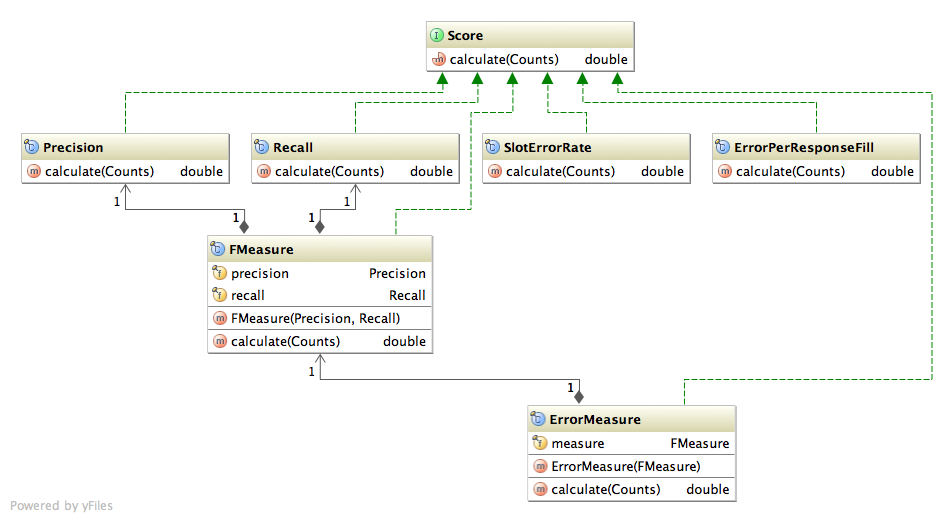
\includegraphics[width=\textwidth, trim=20px 20px 0 0, clip=true]{score.png}
\caption{Score implementation}
\end{figure}

Listing \ref{lst:recall} shows an example \texttt{Score} implementation, in this case \texttt{Recall}.

\begin{listing}[H]
\begin{minted}{java}
final class Recall implements Score {

    @Override
    public double calculate(Counts counts) {
        final double sum = counts.getTruePositives() + 
            counts.getFalseNegatives();

        if (sum > 0) {
            return counts.getTruePositives() / sum;
        } else {
            // cannot divide by zero, return error code
            return Double.NaN;
        }
    }

}
\end{minted}
\caption{Recall score implementation}
\label{lst:recall}
\end{listing}

\newpage
\subsubsection{Performance evaluation}
\begin{figure}[H]
\centering
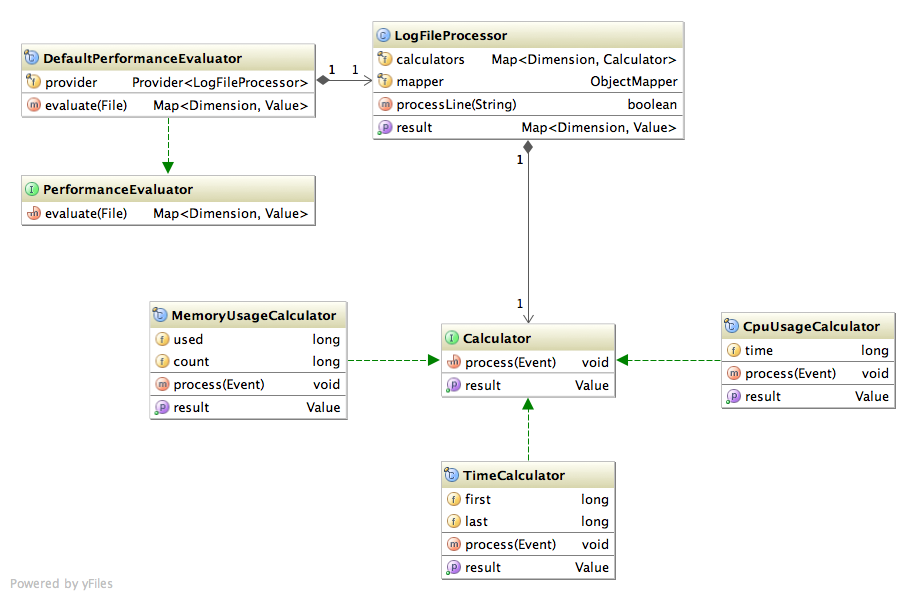
\includegraphics[width=\textwidth, trim=20px 20px 0 0, clip=true]{performance-evaluation.png}
\caption{PerformanceEvaluator implementation}
\end{figure}

Runtime performance evaluation is a little bit easier than quality evaluation. The default \texttt{PerformanceEvaluator} implementation needs to read the event log file line by line, deserialize events, update all configured calculators and finally collect their results.

\begin{listing}[H]
\begin{minted}{java}
@Override
public boolean processLine(String line) throws IOException {
    final Event event = mapper.readValue(line, Event.class);

    for (Calculator calculator : calculators.values()) {
        calculator.process(event);
    }

    return true;
}
\end{minted}
\caption{LogFileProcessor}
\end{listing}

A \texttt{Calculator} is similar to the \texttt{Score} interface shown earlier, except that calculators are inherently stateful.

\begin{listing}[H]
\begin{minted}{java}
interface Calculator {

    void process(Event event);

    Value getResult();

}
\end{minted}
\caption{Calculator Interface}
\label{lst:calculator}
\end{listing}

\fxfatal{At least name all written calculators and their purpose}

Listing \ref{lst:memory-calculator} demonstrates a common \texttt{Calculator} implementation at the example of the \texttt{MemoryUsageCalculator} which computes the average memory consumption in megabytes.

\begin{listing}[H]
\begin{minted}{java}
final class MemoryUsageCalculator implements Calculator {

    private long used;
    private long count;

    @Override
    public void process(Event e) {
        if (e instanceof MemoryUsageEvent) {
            final MemoryUsageEvent event = 
                MemoryUsageEvent.class.cast(e);

            used += event.getValue() / 1024L / 1024L;
            count++;
        }
    }

    @Override
    public Value getResult() {
        return new SimpleValue(used / count);
    }

}
\end{minted}
\caption{MemoryUsageCalculator}
\label{lst:memory-calculator}
\end{listing}
%\section{Results and Analysis}
\label{sec:analysis}

\fxfatal{Results and Analysis}

\subsection{Examples}

\subsection{Scenarios}

\subsection{Comparison}
\section{Conclusion}
\label{sec:conclusion}
This chapter summarizes the work with a review and discusses some lessons learned in the process. It also gives an outlook for future work and research that can be done based on the results of this thesis.

\subsection{Review}
The main objective of this thesis, make an extensible, modular benchmarking framework, has been achieved. So, as a result, we have a prototype Open Source Java-based framework for evaluating and benchmarking information extraction systems which runs in any \gls{OSGi}-compliant environment or embedded as a library in standalone applications.

Additionally I gave an overview over the current state of \gls{IE} , the most common \gls{IE} methods and approaches as well as an introduction to \gls{IE} evaluation methodology. We discussed different matching rules, mapping algorithms and performance and runtime performance measures for evaluating information extraction systems.

The delivered framework prototype currently supports the \textit{All Occurences} \gls{IE} approach and mixed rule approach (\enquote*{contains} and \enquote*{overlap}) for matching reference answers and predictions. It includes, but is not limited to, six different performance (precision, recall, F-Measure, Error measure, Error per response fill and slot error rate) and two runtime performance measures (CPU time and memory consumption). The current version of the software is limited to \acs{JVM}-based extractors, due to the fact that the collecting of the runtime performance measures is realized using \acs{JMX} tools.

The platform was planned to include a web based user interface which provides HTTP uploads for IE programs, monitoring execution progress as well as statistics and scores in form of diagrams. Unfortunately, due to time management issues, this feature has not been realized.

\subsection{Lessons learned}
Modularity is very common buzzword in software engineering, but as so often it's easier said than done. Writing modular software is not easy. It's an ongoing process which consists of continuous dependency management. One needs to split up and introduce levels of indirection to break up too tightly coupled modules. What even makes writing modular software more difficult is that there is no perfect way for modularity, every decission is a compromise between more coarse-grained, and easier to use, modules and more fine-grained, and easier to reuse, modules.  But on the other hand good modular architectur is very similar to good class/package level design, you get used to it and apply patterns without even realizing you are doing so.

Evaluating information extraction systems uniformly is not an easy task either. First of all, very much like the area of \gls{IE} itself, the process of evaluating is as inexact, because there is no general agreement about correct answers of extraction. The desired results differ from domain to domain and even from use case to use case. There might always be a human factor involved in \gls{IE} evaluation to define gold standards for extraction results, since it's so highly subjective.

Another reason why it's difficult to evaluate different tools is the need to find a common data format for extractors which, on the one hand, is simple enough to be adapted to but, on the other hand, flexible enough to handle different \gls{IE} approaches and tasks. Filling templates, see \acl{OBD}, and annotating tokens in a document, see \acl{AO}, are two relatively different approaches and offering a single output format capable of supporting both approaches is not straightforward.

Writing adapters for existing \gls{IE} tools to run and test them in Banshie is not particularly hard but still necessary. The APIs of the selected extractors were reasonable simple to understand and adapt to the framework's interface specification. But different systems and their respective APIs might be more difficult.

\subsection{Outlook and future work}
Banshie's architectural design is based on solid, state-of-the-art patterns, but to expand the framework's capabilities beyond prototype character several ideas come to mind. Some of these ideas will be explained and discussed on the following pages.

The current focus is clearly the field of \textit{Named Entity Recocgnition}, which is an important part of \textit{Information Extraction} and \textit{Natural Language Processing}, but there are other tasks in \gls{IE} which are equally interesting, e.g. relationship extraction, part-of-speech tagging or grammatical sentence analysis (see chapter \ref{sec:information-extraction}).

Supporting multiple \gls{IE} tasks requires Banshie to offer a more flexible XML schema. Reusing the reference- and hypothesis schema definitions proposed by GeMap comes to mind \cite{Linsmayr:2010b}.

Since Evaliex uses a different reference-hypothesis association algorithm, offering a swappable reference-hypothesis mapping algorithm for the performance evaluation could be a useful extension to the framework in order to compare results and/or to allow users to choose based on their use case.

The modified version of the \textit{General Greedy Mapping Algorithm} used in \textit{Evaliex} is based on string/word similarity. Future versions of the Banshie platform should support multiple algorithm, e.g. Levenshtein distance and Jaccard coefficient, as well as a plug-in mechanism for those similarity checks.

The current version of the framework only supports \gls{JVM}-based extractors and since different extractors have different requirements, e.g. memory and garbage collector configuration, applying additional custom command line parameters to the external Java process would be handy too.

Another stage of expansion would include alternate \texttt{Engine} implementations to support non \gls{JVM}-based extractors. Different engines would of course require different means to collect runtime events. In other words for different engines one needs to supply a viable \gls{JMX} client alternative.

The framework, in its current state, is solely an \gls{API}-based tool, which offers great embeddability for \gls{OSGi}- and likewise Java SE environments. To support more use cases providing a simple text-based \gls{CLI} seems to be a promising extension to the platform.

A Web \gls{UI}, in addition to the \gls{CLI}, would be an even more user-friendly approach. A web-based frontend could include fail-safe, responsive and intuitive interface elements to allow easy upload, querying and execution of extractors. A Web \gls{UI} would also be an excellent place to provide visual representations of statistical data and analytical results in the form of charts and diagrams.

Collecting, persisting and aggregating CPU time and memory consumption is the straigtforward approach to measure the runtime performance of a program. But other users might require different or additional measures like file system consumption, thread count or startup latency. \gls{JMX} supports many, many more indicators which could be used by alternative \textit{event production} implementations.

The memory consumption is calculated as the average heap size while the CPU time just looks at the last value. Those are just concrete implementations of generic aggregate functions: \texttt{AVG} and \texttt{LAST} in that case. A more sophisticated approach would be to support an extensible core set of aggregate functions, e.g. \texttt{MIN}, \texttt{MAX}, \texttt{AVG}, \texttt{STDDEV}, \texttt{VAR}, \texttt{SUM}, \texttt{FIRST} and \texttt{LAST}, which operate on the raw logging data. Even offering a lightweight MapReduce integration for a more flexible and user-oriented statistical analysis is imaginable.

\newpage
\addcontentsline{toc}{section}{References}
\nocite{*}
\printbibliography

\printglossaries

\newpage
\addcontentsline{toc}{section}{List of Figures}
\listoffigures

\newpage
\addcontentsline{toc}{section}{List of Tables}
\listoftables

\newpage
\addcontentsline{toc}{section}{List of Listings}
\renewcommand\listoflistingscaption{List of Listings}
\listoflistings

\newpage
\appendix


\end{document}